\documentclass[conference]{IEEEtran}
\IEEEoverridecommandlockouts
% The preceding line is only needed to identify funding in the first footnote. If that is unneeded, please comment it out.
\usepackage{cite}
\usepackage{hyperref}

\usepackage{amsmath,amssymb,amsfonts}
\usepackage{algorithmic}
\usepackage{graphicx}
\graphicspath{ {./images/} }
\usepackage{textcomp}
\usepackage{xcolor}
\hypersetup{
    linkcolor=black
}
\def\BibTeX{{\rm B\kern-.05em{\sc i\kern-.025em b}\kern-.08em
    T\kern-.1667em\lower.7ex\hbox{E}\kern-.125emX}}
\begin{document}

\title{Towards Equitable Collaboration in Pair Programming\\

\author{\IEEEauthorblockN{Valeriia Stromtcova}
\IEEEauthorblockA{\textit{University of Passau}\\
Passau, Germany \\
stromt01@ads.uni-passau.de}}
}

\maketitle

\begin{abstract}
Prior research suggests that pair programming is a highly beneficial tool for students. One of the core principles of PP is that partners in a pair should be equal and active participants. However, not much is known about how pairs are usually formed, and how the level of equity in pairs influences the outcomes of pair programming.

This research paper seeks to study the concept of equity in pair programming. The author aims to find ways to maximize the level of equity in pairs of students who practice pair programming together. To do so, the author conducts a survey among both teachers and students who practice PP. Then, an analysis of the survey results helps to find a relation between pair equity and positive outcomes of pair programming. The author draws conclusions from these results. Lastly, these conclusions serve as a base for recommendations to teachers who use PP as one of the teaching methods.

This study can have an impact on the approach that teachers take while distributing students into pairs for programming. The recommendations given in this paper provide a base to help teachers and students to increase the productivity and quality of collaboration in PP.

\end{abstract}

\begin{IEEEkeywords}
pair programming, collaboration, equity
\end{IEEEkeywords}

\section{Introduction}
Pair programming (PP) refers to a method used in industrial software development or education. As part of this method, two people work together at one computer, aiming to solve a common task. Usually, these two people (employees or students) take turns in the roles of driver and navigator. The driver actively interacts with a computer, coding or designing a piece of work. The navigator watches the working process of their partner and provides feedback. 

Pair programming has numerous positive effects both in industry and in academia. It can increase performance, productivity and quality of code. In the educational environment, it can help achieve better academic performance and a higher student satisfaction rate. However, the outcomes of pair programming can highly depend on how pairs are formed for this type of activity. Typically in the educational environment, a teacher distributes the group of students into pairs to complete programming tasks together. To the author's knowledge, up to this point, there was no research on how teachers perform this distribution of students into pairs and which principles drive this division. Is this process random? Are teachers guided by intuition or some logical considerations? How does this process influence the outcomes of a pair programming task? All these are questions still unanswered by the previous studies.

Both partners in a pair should, in the perfect scenario, be equal and actively participate in the discussion of their task, as well as try to continuously improve their common solution. It means that the collaboration between partners should be as equitable as possible. Educational equity is extremely important for the students and allows everyone to have access to knowledge and resources in the educational environment. But to what extent do teachers consider the concept of equity when dividing student groups into pairs for PP? 

The relation between equitable collaboration and pair programming is not yet well studied and presents a gap in the existing research. This relation becomes the subject of this paper. The author seeks to address the following questions:
\begin{enumerate}
    \item Which methods are currently used by teachers when dividing students into pairs for pair programming and is equity taken into account?
    \item Does the way in which pairs are formed influence the outcomes of pair programming tasks for students? 
    \item How to form pairs in pair programming to promote equitable collaboration between students?
\end{enumerate}

Answering these questions can provide teachers and students applying pair programming for educational purposes with an opportunity to positively influence the results of pair programming tasks and bring more equity into the classroom. The findings will give teachers a theoretical base to divide students into pairs with the aim to maximize level of equity in pairs and thus improve the students' pair programming experience.

\section{Related Work}
According to a recent systematic review of 74 empirical studies of PP, it has numerous positive effects on the outcomes of student learning \cite{HawlBern}. Among these, researchers name improved programming efficiency, increased students' satisfaction and better academic performance \cite{HawlBern}. However, the same study demonstrates that there are gaps in this research field. For instance, there is a "lack of studies focusing on pair compatibility factors aimed at making PP an effective pedagogical tool" (as stated in Hawlitschek et al., 2022 \cite{HawlBern}).

One of such compatibility factors could be equity in education. This concept has been explored in prior studies, e.g. by Ling \& Nasri, 2019 \cite{LingNasr}. According to them, it "is a measure of education achievement such that every individual student is given fair treatment and opportunity to be successful" (as stated in Ling \& Nasri, 2019 \cite{LingNasr}). Earlier studies suggested different definitions of equity, e.g. \cite{ParsTurn} say that equity relates to the distribution of resources between people according to their needs. However, in the current research we will focus on the more modern definition of equity given by Ling \& Nasri, 2019.

Equitable collaboration is a concept based on the principles of equity. Recent research, e.g. by Jeon et al., 2021 \cite{JeonHolm}, defines it in more detail. In equitable educational collaboration, all students have complete access to the conversational floor and are acknowledged in their authority by their group \cite{JeonHolm}. This provides everyone with equal access to knowledge and skills and ensures that everyone has the same possibilities in the educational environment. 

However attractive educational equity might sound, the opposite emerges very often. Research shows that various factors can lead to inequity in student environments. Noltemeyer et al., 2012 \cite{NoltMuji} indicate that race and ethnicity, linguistic diversity, gender and disabilities of students all play a role in the development of educational unequity. Another example is Tesfamicael \& Ayalew, 2021 that suggested that access to quality education for children from developing countries strongly depends on their families' socio-economical status and place of living \cite{TesfAyal}. Another source of inequity in education may be, according to Ling \& Nasri, 2019, differences in digital competences between students \cite{LingNasr}.

The relation between equitable collaboration and pair programming is an emerging field that rarely attracts scientists' attention. The most relevant work in this area by Lewis \& Shah, 2015 \cite{LewiShah} and 2014 \cite{ShahLewi} explores levels of equity in pairs of sixth-grade computer science students and behavioural patterns in these pairs. The analysis combining quantitative and qualitative methods focused on the behaviour of four pairs of students and revealed that inequity in pairs led to marginalization and domination with the focus on completing the tasks as quickly as possible. Therefore, in this study authors suggest that less equitable pairs are prone to increased efficiency (if the metric for efficiency is speed). However, the authors do not explore the relation between equity and students' satisfaction or academic performance. 

\section{Methods}

\subsection{Survey development}

(TODO: explain domination, acknowledgment, role switching)

\subsubsection{Types of questions}

The surveys developed contain both closed-form and open questions. The closed-form questions allow for a quantitative analysis. In most of these questions, the Likert scale \cite{Likert} is used to accurately capture participants' attitude and avoid bias in the formulation of the question itself.

\subsubsection{Survey for students}

The goal of the student survey is to find out how students' experience with pair programming influenced their study outcomes. A list of questions was designed to understand how their pair programming process went with the focus on equity features, and how their academic performance and satisfaction changed over the course of their studies. As a metric of equity, the distribution of talk in pairs is used, similar to the work of Lewis \& Shah, 2015 \cite{LewiShah}.

Below is the list of questions that comprises the survey:

Q1. Have you ever practiced pair programming as part of your studies?
    \begin{itemize}
        \item Yes. The respondent is redirected to Q2.
        \item No. The respondent is redirected to Q2*.
    \end{itemize}

Q2*. You mentioned that you never practiced pair programming as part of your studies. What's your attitude towards trying it out?
    \begin{itemize}
        \item 1 - Very negative
        \item 2 - Negative
        \item 3 - Neutral
        \item 4 - Positive
        \item 5 - Very positive
    \end{itemize}

Q3*. Please explain your choice in the previous question.
    
An alert is shown to the respondent saying:
"If you have practiced pair programming more than once, please focus on \textbf{only one case of pair programming} that you have experienced and that you remember the best. It may be the most recent case of pair programming. Please concentrate on this case and answer the following questions based only on this one case".

Q2. At which stage of your education did you practice pair programming?
    \begin{itemize}
        \item School
        \item University
        \item Extracurricular courses
    \end{itemize}

Q3. How would you estimate your experience with that specific case of pair programming? On a scale from 1 to 5, where 1 is very negative and 5 is very positive. 
    \begin{itemize}
        \item 1 - Very negative
        \item 2 - Negative
        \item 3 - Neutral
        \item 4 - Positive
        \item 5 - Very positive
    \end{itemize}
    
Q4. Please explain your choice in the previous question.  
    
Q5. Choose the most \textbf{positive} aspect in that specific case of programming.
    \begin{itemize}
        \item Communication with my partner
        \item Level of complexity of the task
        \item Speed of completion of the task
        \item Teacher's guidance
        \item Better memorization of the material
    \end{itemize}
    
Q6. Choose the most \textbf{negative} aspect in that specific case of pair programming.
    \begin{itemize}
        \item Communication with my partner
        \item Level of complexity of the task
        \item Speed of completion of the task
        \item Teacher's guidance
        \item Worse memorization of the material
    \end{itemize}
    
Q7. Did you feel like your partner or you dominated the conversational floor, expressing ideas and making suggestions more often?
    \begin{itemize}
        \item 1 - I expressed my ideas way more often than my partner.
        \item 2 - I expressed my ideas slightly more often than my partner.
        \item 3 - Both me and my partner expressed their ideas equally often.
        \item 4 - My partner expressed their ideas slightly more often than me.
        \item 5 - My partner expressed their ideas way more often than me.
    \end{itemize}

Q8. In pair programming, the driver actively interacts with a computer, coding or designing a piece of work. The navigator watches the working process of their partner and provides feedback. Did you and your partner only do what is prescribed by your roles?
    \begin{itemize}
        \item Yes, we have both been sticking to our roles.
        \item No, my partner sometimes took my role.
        \item No, I sometimes took the role of my partner.
        \item No, we both did something that was not prescribed by our roles.
        \item I am not sure.
    \end{itemize}

Q9. To what extent do you feel, overall, like your ideas and suggestions are appreciated and taken into account by your pair programming partner?
    \begin{itemize}
        \item 1 - My partner did not listen to me and appreciate my comments at all.
        \item 2 - My partner mostly did not listen to me and appreciate my comments.
        \item 3 - My partner sometimes listened to me and appreciated my comments and sometimes not.
        \item 4 - My partner most of the time listened to me and appreciated my comments.
        \item 5 - My partner always listened to me and appreciated my comments.
    \end{itemize}

Q10. Is anything of the following true regarding you and your pair programming partner? (multiple choice)
    \begin{itemize}
        \item We belonged to the same gender group.
        \item We belonged to the same ethnicity.
        \item We belonged to the same age group (+-5 years)
        \item We possessed (almost) the same level of digital competency
        \item None of the above.
    \end{itemize}
    
Q11. How did this specific case of pair programming influence your academic performance?
    \begin{itemize}
        \item 1 - Very negative influence
        \item 2 - Negative influence
        \item 3 - Neutral influence
        \item 4 - Positive influence
        \item 5 - Very positive influence
    \end{itemize}
    
Q12. Do you think that pair programming is supportive of equity between students?
    \begin{itemize}
        \item 1 - Not at all.
        \item 2 - A bit.
        \item 3 - Neither yes, neither no.
        \item 4 - Supportive.
        \item 5 - Extremely supportive.
    \end{itemize}

\subsubsection{Survey for teachers}

The goal of the teacher survey is to find out how they divide students into groups for pair programming, and how they estimate the pair programming outcomes for their students. 

Below is the list of questions that comprises the survey:

Q1. Have you ever user pair programming as one of your teaching methods?
    \begin{itemize}
        \item Yes. The respondent is redirected to Q2.
        \item No. The respondent is redirected to Q2*.
    \end{itemize}

Q2*. You mentioned that you never used pair programming as one of your teaching methods. What's your attitude towards trying it out?
    \begin{itemize}
        \item 1 - Very negative
        \item 2 - Negative
        \item 3 - Neutral
        \item 4 - Positive
        \item 5 - Very positive
    \end{itemize}

Q3*. Please explain your choice in the previous question.

An alert is shown to the respondent saying:
"If you have given pair programming tasks to your students more than once, please focus on \textbf{only one case of pair programming} that you remember the best. It may be the most recent case of pair programming. Please concentrate on this case and answer the following questions based only on this one case".

Q2. Why did you introduce pair programming in your class?

Q3. At which stage of education did your students practice pair programming with you?
    \begin{itemize}
        \item School
        \item University
        \item Extracurricular courses
    \end{itemize}

Q4. How would you estimate your experience with that specific case of pair programming? 
    \begin{itemize}
        \item 1 - Very negative
        \item 2 - Negative
        \item 3 - Neutral
        \item 4 - Positive
        \item 5 - Very positive
    \end{itemize}
    
Q5. Please explain your choice in the previous question.  

Q6. Which of the following aspects, if any, did you consider while distributing your students into pairs for pair programming?
    \begin{itemize}
        \item Gender
        \item Ethnicity
        \item Age
        \item Digital competency
        \item None of the above
    \end{itemize}

Q7. How specifically did you consider the gender aspect when dividing students into pairs? (this question is only shown if the respondent chose gender as one of the answers in Q6)
    \begin{itemize}
        \item I tried to make pairs diverse with regards to gender (paired male with female).
        \item I tried to make pairs homogeneous with regards to gender (paired male with male, female with female).
    \end{itemize}

Q8. How specifically did you consider the ethnicity aspect when dividing students into pairs? (this question is only shown if the respondent chose ethnicity as one of the answers in Q6)
    \begin{itemize}
        \item I tried to make pairs diverse with regards to ethnicity (paired people of different ethnicities).
        \item I tried to make pairs homogeneous with regards to ethnicity (paired people of same ethnicities).
    \end{itemize}

Q9. How specifically did you consider age when dividing students into pairs? (this question is only shown if the respondent chose age as one of the answers in Q6)
    \begin{itemize}
        \item I tried to make pairs diverse with regards to age (paired students of different ages).
        \item I tried to make pairs homogeneous with regards to gender (paired students of close ages).
    \end{itemize}

Q10. How specifically did you consider digital competency when dividing students into pairs? (this question is only shown if the respondent chose digital competency as one of the answers in Q6)
    \begin{itemize}
        \item I tried to make pairs diverse with regards to digital competency (paired students of different digital competency levels).
        \item I tried to make pairs homogeneous with regards to digital competency (paired students of close digital competency levels).
    \end{itemize}
    
Q11. When observing pairs of students, did you see cases where a student dominates over his/her partner in the discussion of the task?
    \begin{itemize}
        \item 1 - I have seen no such cases.
        \item 2 - There were few such cases.
        \item 3 - 50\% of pairs had patterns of domination, the other ones didn't
        \item 4 - There were many such cases.
        \item 5 - All pairs showed patterns of domination.
    \end{itemize}

Q12. When observing pairs of students, did you see cases where a students did not follow the rules regarding role responsibilities?
    \begin{itemize}
        \item 1 - I have seen no such cases.
        \item 2 - There were few such cases.
        \item 3 - 50\% of pairs had patterns of role switching, the other ones didn't
        \item 4 - There were many such cases.
        \item 5 - All pairs showed patterns of role switching.
    \end{itemize}
    
Q13. Do you think that pair programming had an impact on students' academic performance?
    \begin{itemize}
        \item 1 - The performance worsened significantly
        \item 2 - The performance worsened slightly
        \item 3 - The performance remained the same
        \item 4 - The performance improved slightly
        \item 5 - The performance improved significantly
    \end{itemize}
    
Q14. Which kind of feedback did students have about the pair programming session?
    \begin{itemize}
        \item 1 - Very negative feedback
        \item 2 - Negative feedback
        \item 3 - Neutral feedback
        \item 4 - Positive feedback
        \item 5 - Very positive feedback
    \end{itemize}

Q15. In your opinion, how supportive of equity is pair programming?
    \begin{itemize}
        \item 1 - Not at all.
        \item 2 - A bit.
        \item 3 - Neither yes, neither no.
        \item 4 - Supportive.
        \item 5 - Extremely supportive.
    \end{itemize}

\subsection{Data collection}

The data is collected with the usage of Prolific platform, a tool that allows to find research participants by various criteria, and SoSci survey platform. The primary target of the surveys are students and teachers who have experience with pair programming. These respondents are more likely to be found in the Computer Science field. Therefore, the first survey targeted 5,683 possible respondents among students on this platform. These people have indicated that they studied either Computer Science or Computing as part of their education program. The filter for teachers was less precise, as Prolific does not have the feature to filter only Computer Science teachers. Instead, two filters were applied: Job is Teacher and Skills include Computer Programming. Based on these criteria, the teacher survey targeted 949 participants.

The survey consists of two parts: prescreen and the survey itself. The prescreen contained only one question for both students and teachers, and the question addressed the usage of pair programming as a tool for either teaching or studying. Only those participants who have practiced pair programming could access the survey itself. Out of 406 students who passed the prescreen phase, 252 participated in the survey and successfully completed it. As for the teachers, the amount of collected data was lower: 303 respondents finished the prescreen, and 82 completed the survey.

\subsection{Data preprocessing}
\begin{table}[h]
    \begin{tabular}{ |c|p{50px}|c| }
        \hline
        Answer type & \# of questions & Preprocessing strategy\\
        \hline
        Free text & 5 for students, 8 for teachers & Manual examination\\
        \hline
        Multiple choice (Likert scale) & 9 for students, 10 for teachers & Encoding as values from 1 to 5\\
        \hline
        Multiple choice (Simple) & 5 for students, 6 for teachers & One-hot encoding \\
        \hline
        Multiple choice (Complex) & 6 for students, 2 for teachers &  \\ 
        \hline
    \end{tabular}
    \caption{Data preprocessing strategies by question type}
    \label{tab:table1}
\end{table}

The data preprocessing strategy for each question depends on the data type received as an answer to that question. Table \ref{tab:table1} displays the choice of a preprocessing strategy for each answer type. The data was preprocessed and later analyzed with the usage of Python programming language, Jupyter Notebook computing platform, Pandas data analysis library and manual effort. The source code for data preprocessing and analysis is available in a public \href{https://github.com/lerastromtsova/pair-programming-equity}{Github repository} \cite{Repository}.

\subsection{Data analysis}
\subsubsection{Hypothesis 1}
Currently teachers rarely take equity into account when dividing students into pairs for PP.

In order to justify or reject this hypothesis, the data from the section "Pair formation" of the teacher survey was closely analysed. Figure \ref{fig:aspectsPairFormation} displays the distribution of different aspects that teachers consider when creating pairs.

\begin{figure}[h]
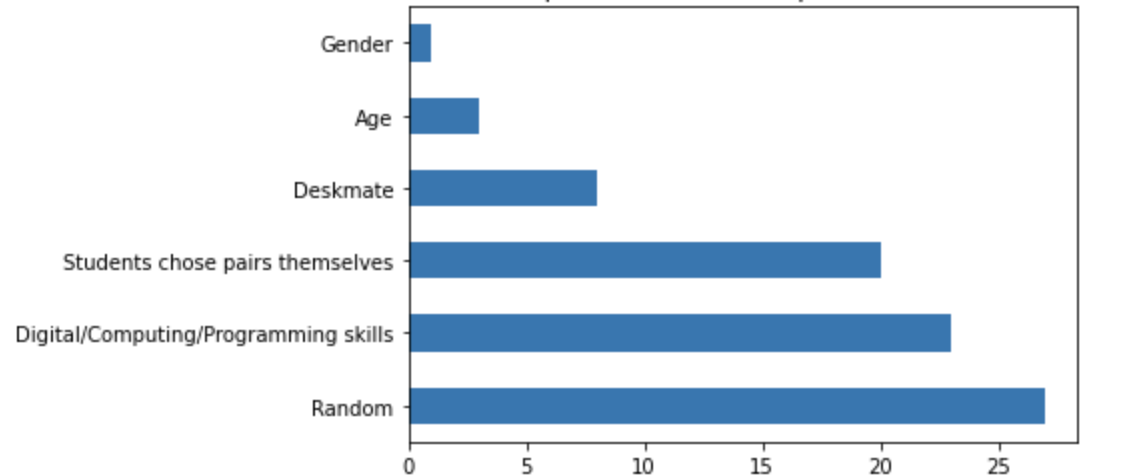
\includegraphics[scale=0.42]{aspects-pair-formation.png}
\caption{Pair formation aspects considered by teachers}
\label{fig:aspectsPairFormation}
\end{figure}

Judging by the survey results, most of the teachers (32\%) distribute students into pairs randomly. Random pair formation, according to the teachers' responses, has the following benefits:

\begin{itemize}
    \item Lets students get out of their comfort zone and interact with different people;
    \item Increases pair diversity;
    \item Provides an easier way for the teachers to distribute students into pairs;
    \item Is considered a fair approach introducing less bias.
\end {itemize}

The second popular approach to distribute students into pairs is to consider their digital competency skills. However, the exact method of taking these skills into account differs drastically for different respondents. Approximately 60\% of the teachers who consider digital competency an important aspect of pair formation tried to make pairs of students diverse with regards to digital competency. Their main justification for such an approach can be summarized as "Strong will help the weak". In other words, these teachers assumed that matching students with diverse skills will lead to more advanced students passing their skills and knowledge to less advanced ones. Another 40\% did the direct opposite and aimed to match students with close levels of digital competency. Those teachers mainly assumed that both students in a pair would benefit from such an approach; some respondents tried to avoid excess domination of one partner over the other.

Another popular approach, used by 24\% of the respondents, was to let students choose the pairs themselves. The reasoning behind this method was the following:
\begin{itemize}
    \item It is more comfortable for students to work with someone they have chosen themselves;
    \item "Students know best": students can make the right choice on who they would like to work with;
    \item Such an approach may increase efficiency or pair work.
\end{itemize}

Overall, out of 83 respondents, \textbf{only 3 have clearly stated} that they have thought about domination and/or acknowledgment patterns in pairs arising from the results of pair formation. We will refer to these respondents as "Group 1". Another \textbf{14 out of 83} ("Group 2") told that they tried to pair "stronger" students with "weaker" ones so that stronger ones teach the weaker ones. However, this approach has major drawbacks: it leads to domination, role switching and low acknowledgment behavioural patterns. This can be clearly seen if we plot the data for these two groups (Figure \ref{fig:dominationCompare}).

\begin{figure}[h]
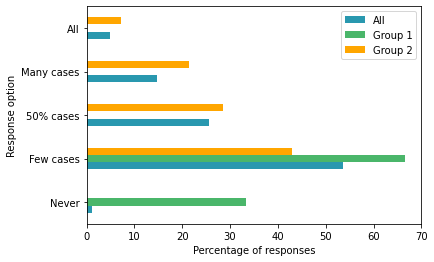
\includegraphics[scale=0.5]{images/domination-comparison.png}
\caption{Frequency of dominational patterns by Groups, Group 1 and 2, respectively}
\label{fig:dominationCompare}
\end{figure}

As can be seen on the chart in Figure \ref{fig:dominationCompare}, Group 1 (marked with green) where teachers tried to avoid domination in pairs achieves a significantly lower level of domination: they either observe dominational patterns in few cases or never. This group of teacher was initally dividing students into pairs considering either age or digital competency and tried to make pairs homogeneous. The reasoning behind that was avoiding domination. Group 2 (marked with orange), in contrast, paired students with different level of digital competencies or used random division into pairs. For this group of teachers, the dominational patterns are observed in much larger proportion of cases than Group 1. When compared with the averaged statistics across all dataset (marked with blue), Group 2 also performs worse than the rest with regards to domination. 

\begin{figure}[ht]
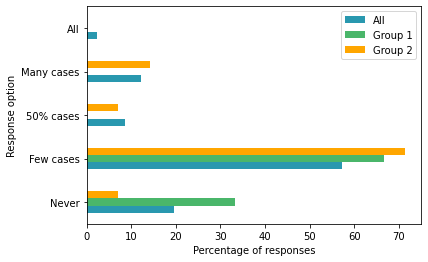
\includegraphics[scale=0.5]{role-switch-comparison.png}
\caption{Frequency of Role Switching patterns by Groups, Group 1 and 2, respectively}
\label{fig:roleSwitchCompare}
\end{figure}

The same pattern emerges when we take a look at the Role Switching pattern for Group 1, Group 2 and all the dataset. Figure \ref{fig:roleSwitchCompare} shows a comparison of these groups and distribution of Role Switching pattern reported by them. Role Switching pattern rarely appears in pairs formed by teachers from Group 1. The frequency of its appearance is higher if averaged across all dataset. Finally, Group 2's performance is much less satisfactory.

\begin{figure}[ht]
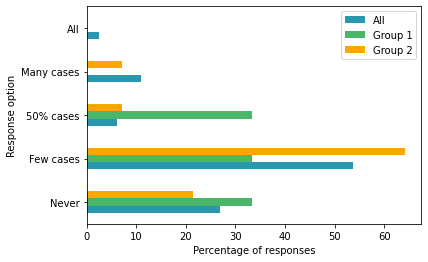
\includegraphics[scale=0.5]{ack-comparison.png}
\caption{Frequency of Acknowledgment patterns by Groups, Group 1 and 2, respectively}
\label{fig:ackCompare}
\end{figure}

Acknowledgment is the only slight exception from the general trend that we noticed when comparing Group 1 and Group 2. Here, Group 2 performs slightly better than Group 1. However, the results for Group 1 are still overall positive, and students generally show acknowledgment of their partners.

This step of data analysis leads to a conclusion even though teachers rarely consider equity while distributing students into pairs, they should probably do so, because it leads to fewer cases of domination and role switching, therefore ensuring a more pleasant experience for their students. 

As a result of this step of data analysis, Hypothesis 1 was confirmed and a recommendation for teachers on the way to distribute students into pairs was formulated.

\subsubsection{Hypothesis 2}
There is a positive correlation between level of equity in pairs and positivity of PP outcomes.

To investigate this hypothesis, data from both teacher and student surveys should be used. 

As for the teacher survey, a correlation matrix for experience- and performance-related answers and behavioural patterns-related answers has been built. Experience- and performance-related answers point at the positivity of PP outcomes, while behaviour-related answers can provide information about levels of equity in pairs. Therefore, a correlation between these groups of answers could identify the correlation between equity and positivity of PP outcomes. Correlation is measured using Pearson's coefficient.

\begin{table}[ht]
    \centering
    \begin{tabular}{|l|r|r|r|r|r|}
    \hline
    {} &      EX01 &      EX03 & PE01 & PE02 & PE03 \\
    \hline
    BP01 & -0.16 & -0.09 & 0.14 & -0.02 & 0.00\\
    \hline
    BP02 & -0.23 & -0.10 & -0.04 & -0.11 & -0.04\\
    \hline
    BP03 & -0.16 & -0.15 & -0.06 & -0.13 & 0.02\\
    \hline
    \end{tabular}
    \caption{Correlation matrix for experience- and performance-related answers and equity-related answers}
    \label{tab:table2}
\end{table}

As can be seen from Table \ref{tab:table2}, no significant correlation was found between all experience- and performance-related data and behaviour-related data. Just a small correlation ranging from -0,23 to 0,14 is present. Therefore, judging from the teachers' data, Hypothesis 2 should be rejected.

\begin{table}[ht]
    \centering
    \begin{tabular}{|l|r|r|r|r|r|}
    \hline
    {} &      EX01 &      EX05 & PE01 & PE02 & PE05 \\
    \hline
    BP01 & -0.26 & -0.27 & -0.15 & -0.12 & -0.10 \\
    \hline
    BP02 & -0.17 & -0.21 & -0.17 & -0.12 & -0.11\\
    \hline
    BP03 &  0.39 &  0.29 & 0.33 & 0.32 & 0.34\\
    \hline
    \end{tabular}
    \caption{Correlation matrix for experience- and performance-related answers and equity-related answers}
    \label{tab:table3}
\end{table}

Taking a look at the student survey (Table \ref{tab:table3}), the correlation coefficients are slightly more significant and range from -0,26 to 0,39. The highest positive correlation observed is between answers to question BP03 (acknowledgment in pairs) and question EX01 (how positive is a student's experience in this specific case of PP). Similar correlation coefficients are obserrved for BP03 and PE01, PE02, PE05. However, as the interpretation of Pearson's coefficient differs across scientific sources, the score of 0,39 can be considered either a weak positive correlation or a moderate positive correlation. In any case, the correlation is not strong enough to reliably support Hypothesis 2.

As a result of this step of data analysis, Hypothesis 2 was rejected. There does not seem to be a strong enough positive correlation between level of equity in PP pairs and the positivity of PP outcomes. 

\subsubsection{Hypothesis 3}
The more homogeneous a pair is with regards to gender, age, ethnicity and digital competency, the higher is the level of equity in this pair.

\begin{table}[ht]
    \centering
    \begin{tabular}{|l|r|r|r|r|r|}
    \hline
    {} &   DI01.01 &   DI01.02 &   DI01.03 &   DI01.04 &   DI01.05 \\
    \hline
    BP01 & -0.04 & -0.16 & -0.07 & -0.31 &  0.11 \\
    \hline
    BP02 & -0.13 & -0.21 & -0.09 & -0.23 &  0.04 \\
    \hline
    BP03 &  0.15 &  0.19 &  0.17 &  0.22 & -0.03 \\
    \hline
    \end{tabular}
    \caption{Correlation matrix for diversity-related answers and equity-related answers}
    \label{tab:table4}
\end{table}

As shown in Table \ref{tab:table4}, the correlation between homogeneity of a pair (represented by data in DI01.01-DI01.05) and equity (measured with BP01-BP03) is insignificant as well. The correlation coefficient ranges from -0,31 to 0,19. The biggest negative correlation is -0,31 for features BP01 and DI01.04. This might indicate some relation between level of digital competency and Domination pattern, meaning that the more homogeneous a pair is in terms of digital competency, the less domination there is in such a pair. However, the correlation is too slight to draw conclusions from it.

Taking a closer look at the data, we can proceed with analysing the DI02 question about the desirable characteristics of a pair programming partner for students.

\begin{figure}[ht]
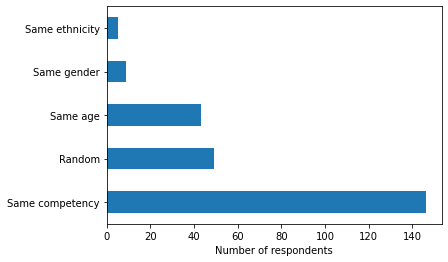
\includegraphics[scale=0.5]{important-attribute.png}
\caption{Importance of different partner attributes for students}
\label{fig:impAttr}
\end{figure}

Figure \ref{fig:impAttr} displays student responses regarding desirable characteristics of their PP partners. 

Most students (58\%) would prefer to have a partner with the same competencies. In DI03, students elaborate on the reasons of choice of this option. Some of them do not want to feel less advanced than their partner; others do not want to explain concepts to their partners; others think that possessing the same level of competency eases communication. Other reasons for choosing this answer include equally sharing the workload, fairness in distributing the tasks, and efficiency in reaching pair programming goals.

Only 19\% of the respondents prefer to be randomly split into pairs. Another 17\% would like to work with partners from the same age group. They name such advantages of this answer as easier communication, increased confidence, and possible domination of the older partner.

The least popular answers among the students were "Same gender" (4\%) and "Same ethnicity" (2\%). The reasoning behind this for these respondents is avoiding domination and increasing acknowledgment between partners. This partially confirms the hypothesis and proves that for at least a small fraction of respondents (6\%) matching based on similar gender and/or ethnicity helps achieve better equity.

Overall, the way in which pairs are formed is important for students. Since only 19\% of the respondents prefer random distribution into pairs, the vast majority (81\%) considers such factors as similar digital competency, age, ethnicity and gender to be beneficial for the pair programming process. The respondents name various reasons for this, sometimes mentioning Domination and Acknowledgment patterns. Based on this data, as well as the correlations provided in the Table \ref{tab:table4}, it can be said that Hypothesis 3 was partially confirmed (for some of the students).

\section{Results}
Hyp 1
Hyp 2
Hyp 3
..
Recommendations for teachers

\section{Discussion}
- Not much data - easier to analyse, especially free text, but may cause a threat to validity
- Indirect estimations (e.g. performance is measured subjectively)
- Typos in questions

\section{Conclusions}
To be done.


\begin{thebibliography}{00}
\bibitem{HawlBern} Hawlitschek, A., Berndt, S., \& Schulz, S. (2022). Empirical research on pair programming in higher education: a literature review. Computer Science Education, 1-29.
\bibitem{LingNasr} Ling, T., \& Nasri, N. M. (2019). A systematic review: Issues on equity in education. Creative Education, 10(12), 3163.
\bibitem{ParsTurn} Parsons, E. C., \& Turner, K. (2014). The importance of history in the racial inequality and racial inequity in education: New Orleans as a case example. Negro Educational Review, 65(1-4), 99.
\bibitem{JeonHolm} Jeon, S., Holmes, N. G., Sayre, E. C., \& Franklin, S. (2021). An Interplay of Problem-Solving Modes and Authority: Framework for Equitable Collaboration in Undergraduate Physics Labs. In Proceedings of the 15th International Conference of the Learning Sciences-ICLS 2021.. International Society of the Learning Sciences.
\bibitem{NoltMuji} Noltemeyer, A. L., Mujic, J., \& McLoughlin, C. S. (2012). The history of inequity in education. Disproportionality in education and special education: A guide to creating more equitable learning environments, 3-22.
\bibitem{TesfAyal} Tesfamicael, S. A., \& Ayalew, Y. (2021). Mathematics education in Ethiopia in the era of COVID-19: Boosting equitable access for all learners via opportunity to learning. Contemporary Mathematics and Science Education, 2(1), 1-9.
\bibitem{LewiShah} Lewis, C. M., \& Shah, N. (2015, August). How equity and inequity can emerge in pair programming. In Proceedings of the eleventh annual international conference on international computing education research (pp. 41-50).
\bibitem{ShahLewi} Shah, N., Lewis, C., \& Caires, R. (2014). Analyzing equity in collaborative learning situations: A comparative case study in elementary computer science. Boulder, CO: International Society of the Learning Sciences.
\bibitem{Likert} Likert, R. (1932). A Technique for the Measurement of Attitudes. Archives of Psychology, 140, 1–55.
\bibitem{Repository} Stromtcova, V. (2022). Pair Programming Equity repository. GitHub. https://github.com/lerastromtsova/pair-programming-equity

\end{thebibliography}
\vspace{12pt}

\end{document}
